\section{Gold-PVD}
\label{goldpvd}

Als Testsystem für PVD-Prozesse bietet sich Gold-PVD an, die zwar durch Oberflächendiffusion dominiert wird, jedoch ideale fcc-kristalline Strukturen bildet.
Die genutzte EAM-Potentialdatei stammt aus dem \todo{ref}LAMMPS-Paket, basiert aber auf Parametern von Foiles et al.\cite{foiles_embedded-atom-method_1986}, die für Einbettung einzelner Atome in Bulk- und Oberflächensysteme optimiert wurden.

\subsection{Voruntersuchungen}

Zur Validierung grundlegender Materialeigenschaften wurden Bindungslängen, Dichten und Koordinationszahlen aus einer relaxierten kristallinen Phase untersucht (Tabelle \ref{tab:goldpreresults}).
Zur Bestimmung dieser Werte wurde ein Goldkristall von \SI{40x40x40}{\angstrom} Größe auf \SI{1000}{\kelvin} aufgeheizt, im kanonischen Ensemble relaxiert und anschließend abgekühlt.
Wie man den Ergebnissen ansehen kann, bleibt die Kristallstruktur erwartungsgemäß erhalten (die Schmelztemperatur wurde für die Relaxierung nicht überschritten) und steht in guter Übereinstimmung mit Literaturwerten.
Die Parametrisierung repräsentiert somit das Zielsystem.

\begin{table}[hbtp]
  %% \rowcolors{0}{white}{lightgray} 
  \caption[Eigenschaften von Gold]{Vergleich der Eigenschaften von Gold mit experimentellen und Literaturdaten als Voruntersuchung des PVD-Prozesses
    %% \todo[inline]{ref}
  }
  \label{tab:goldpreresults}
  \begin{tabularx}{\textwidth}{|lXXXX|}
    \hline
    \textbf{unters. Größe} & \textbf{Temperatur} & \textbf{Simulation} & \textbf{Experiment} & \textbf{Abweichung}\\
    \hline
    Bindungslänge  &  \SI{50}{\kelvin}   &  \SI{2.885}{\angstrom}                    &  \SI{2.884}{\angstrom}                    &  \SI{0.05}{\percent}  \\
    Koordination   &  \SI{50}{\kelvin}   &  \SI{12.00}{}                             &  \SI{12.00}{}                             &  \SI{0}{\percent}     \\
    Dichte         &  \SI{300}{\kelvin}  &  \SI{18.99}{\gram\per\cubic\centi\meter}  &  \SI{19.30}{\gram\per\cubic\centi\meter}  &  \SI{1.6}{\percent}   \\
    Dichte         &  \SI{500}{\kelvin}  &  \SI{18.89}{\gram\per\cubic\centi\meter}  &  \SI{19.13}{\gram\per\cubic\centi\meter}  &  \SI{1.2}{\percent}   \\
    \hline
  \end{tabularx}
\end{table}

%% \todo[inline]{Oberflächenvalidierung}

\subsection{Thermodynamische Eigenschaften}

Neben strukturellen Eigenschaften bilden EAM-Potentiale auch einige thermodynamische Eigenschaften von Metallen ab.
Für deren Untersuchung wurde die Massendichte in Abhängigkeit der Temperatur für die Teststruktur aufgenommen, die langsam auf \SI{2000}{\kelvin}, also weit über den Schmelzpunkt von \SI{1337}{\kelvin}, aufgeheizt wurde.
Die Ergebnisse (Abbildung \ref{fig:goldthermo}) zeigen gute Übereinstimmung mit experimentellen Daten, wofür Relaxationszeiten $t_\text{relax}$ oberhalb von \SI{20}{\pico\second} und Thermostat-Dämpfungsparameter $D_T$ \SI{\approx0.02}{\femto\second} als notwendig ermittelt wurden.
Bei geringeren $t_\text{relax}$ oder $D_T$ relaxiert das System innerhalb eines Temperaturschrittes nicht vollständig, wodurch der Schmelzpunkt überschätzt wird, wie in Abbildung \ref{fig:goldthermo-b} zu sehen ist.

\begin{figure}
  \captionsetup[subfigure]{singlelinecheck=false}
  \def\subfigwidth{7cm}
  \begin{subfigure}[t]{\subfigwidth}
    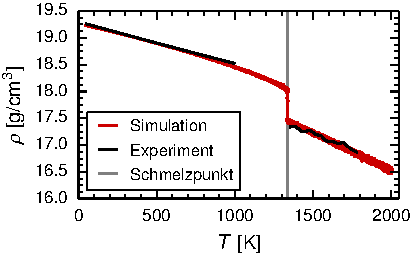
\includegraphics[width=\textwidth]{gold_bestthermo}
    \subcaption{Temperaturverlauf bei $ t_\text{relax}=\SI{50}{\pico\second}$ und $D_T=\SI{0.02}{\femto\second}$}
    \label{fig:goldthermo-a}
  \end{subfigure}
  \hfill
  \begin{subfigure}[t]{\subfigwidth}
    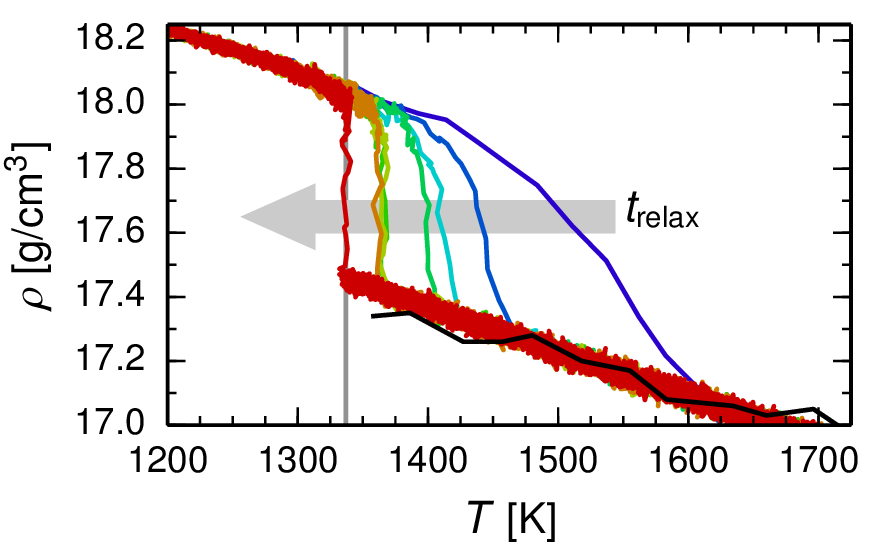
\includegraphics[width=\textwidth]{gold_relaxtime}
    \subcaption{Abhängigkeit des simulierten Schmelzpunktes von der Relaxationszeit}
    \label{fig:goldthermo-b}
  \end{subfigure}
  \caption[Ergebnisse thermodynamischer Simulationen von Gold]{Ergebnisse thermodynamischer Simulationen von Gold.
    Verlauf stimmt gut mit experimentellen Daten (schwarze Linien) überein.
    Experimentelle Werte stammen aus Standardliteratur sowie von Brillo et al.\cite{brillo_density_2006}.
  }
  \label{fig:goldthermo}
\end{figure}

\subsection{Prozess-Simulation}

Zur Simulation eines Gold-PVD-Prozesses mit Parsivald wurden die untersuchten Potentialparameter sowie ein Kristallsubstrat im PVD-Modus eingelesen und Relaxationszeiten und Reaktionsnachbarschaftsgrößen aus den Vorbetrachtungen übernommen.
Damit ergeben sich Reaktionsräume der Größe \SI{37x37x25}{\angstrom} mit jeweils ca. \num{1800} Atomen, Relaxationszeiten von \SI{1.4}{\nano\second} in \num{1400} Simulationsschritten und Auftreffgeschwindigkeiten von \SI{4}{\angstrom/\pico\second}, die aus üblichen Sputterbedingungen stammen.\todo{wie berechnet?}

Abbildung \ref{fig:golddepositions-a} zeigt, wie das Substrat unter Erhalt der Kristallstruktur fortgesetzt wird.
Poren und Einschlüsse wurden durch Untersuchung der Alphastruktur nicht gefunden.
Abbildung \ref{fig:goldroughness-a} stellt die Rauheit dar, die beim glatten Substrat über den Abscheidungszeitraum konstant geblieben ist.
Fehler- und Abbruchsquoten bei den LAMMPS-Berechnungen lagen mit \SI{0.25}{\percent} unterhalb des aus den ALD-Prozessen der Bachelorarbeit erwarteten Wertes von \SI{5}{\percent}

\subsubsection{Wachstum auf strukturierten Substraten}

Neben dem glatten Substrat wurden auch Abscheidungen auf strukturierten Substraten (Abbildung \ref{fig:golddepositions}) mit den gleichbleibenden Prozessbedingungen simuliert.
Als Substrate wurden Stufen oder Spitzen mit einer Höhe von jeweils \SI{20}{\angstrom} und Neigungen von \SI{15}{\degree}, \SI{20}{\degree}, \SI{30}{\degree}, \SI{45}{\degree}, \SI{60}{\degree} und \SI{90}{\degree} präpariert.
Auf vorherige Relaxierung der Substrate wurde aufgrund der Prozessstabilität sowie der relaxierenden Eigenschaften der MD-Ereignisse verzichtet.
Zusätzlich wurden Lamellen und Gitter mit einer Strukturbreite von \SI{16}{\angstrom} zur Untersuchung eventueller Prozessartefakte präpariert.

\begin{figure}[p]
  \captionsetup[subfigure]{singlelinecheck=false}
  \def\subfigwidth{0.31\textwidth}
  \begin{subfigure}[t]{\subfigwidth}
    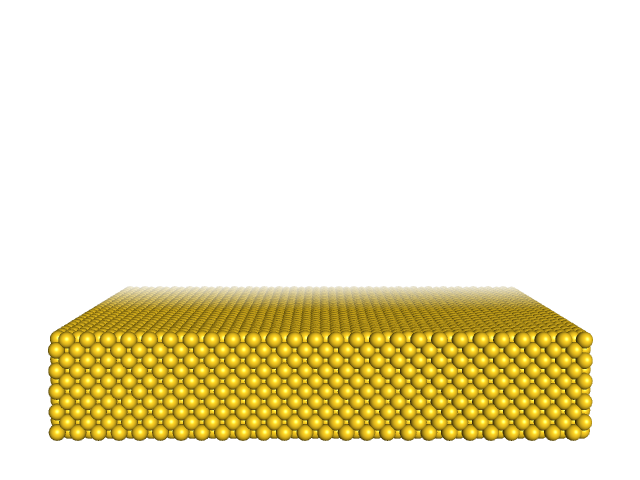
\includegraphics[width=\textwidth]{Au_substrate_flat}
    \subcaption{Glattes Gold-Substrat}
    \label{fig:golddepositions-a}
  \end{subfigure}
  \hfill
  \begin{subfigure}[t]{\subfigwidth}
    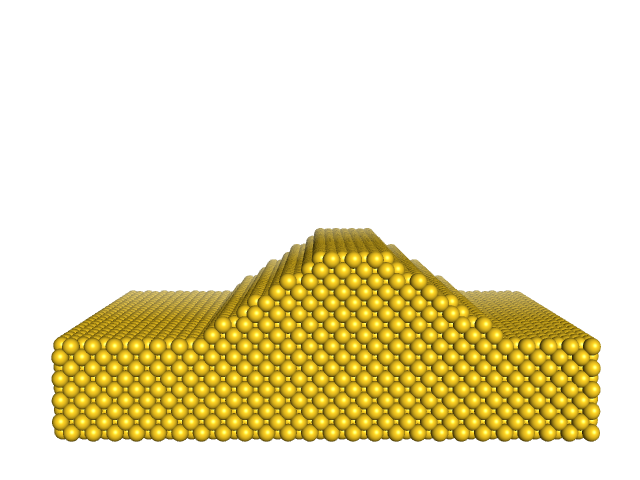
\includegraphics[width=\textwidth]{Au_substrate_step30}
    \subcaption{Gold-Stufe, \SI{30}{\degree}}
    \label{fig:golddepositions-b}
  \end{subfigure}
  \hfill
  \begin{subfigure}[t]{\subfigwidth}
    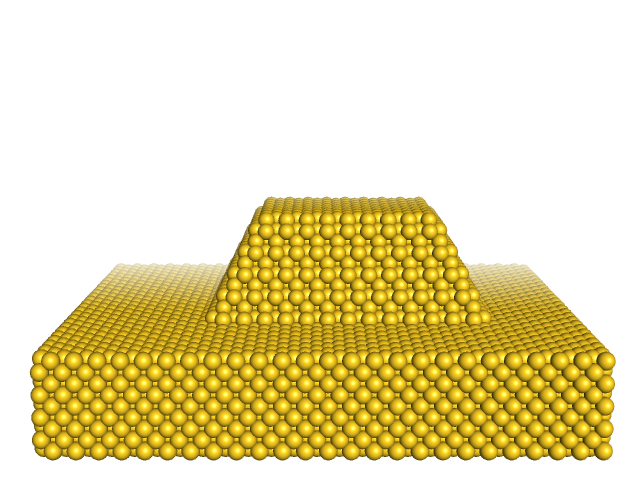
\includegraphics[width=\textwidth]{Au_substrate_tip60}
    \subcaption{Gold-Spitze, \SI{60}{\degree}}
    \label{fig:golddepositions-c}
  \end{subfigure}

  \Large\center{$\Downarrow$}
  \vspace{0.25cm}

  \captionsetup[subfigure]{singlelinecheck=false}
  \def\subfigwidth{0.31\textwidth}
  \begin{subfigure}[t]{\subfigwidth}
    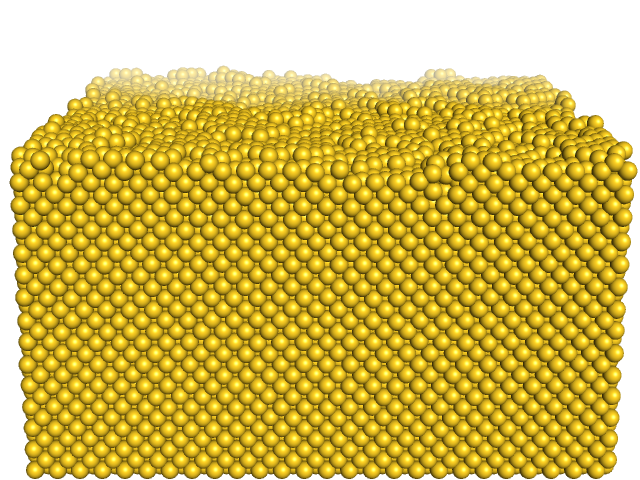
\includegraphics[width=\textwidth]{Au_deposition_flat}
    \subcaption{Glatte, kristalline Schicht ($\sigma_z = \SI{1.2}{\angstrom}$)}
    \label{fig:golddepositions-d}
  \end{subfigure}
  \hfill
  \begin{subfigure}[t]{\subfigwidth}
    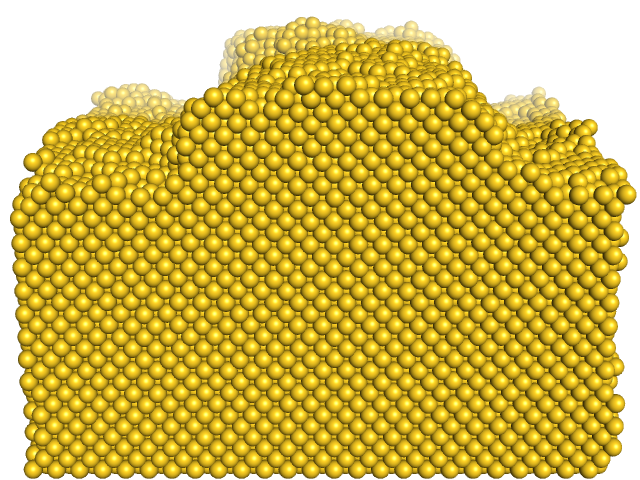
\includegraphics[width=\textwidth]{Au_deposition_step30}
    \subcaption{Fortsetzung der Stufe ($\sigma_z = \SI{6.4}{\angstrom}$)}
    \label{fig:golddepositions-e}
  \end{subfigure}
  \hfill
  \begin{subfigure}[t]{\subfigwidth}
    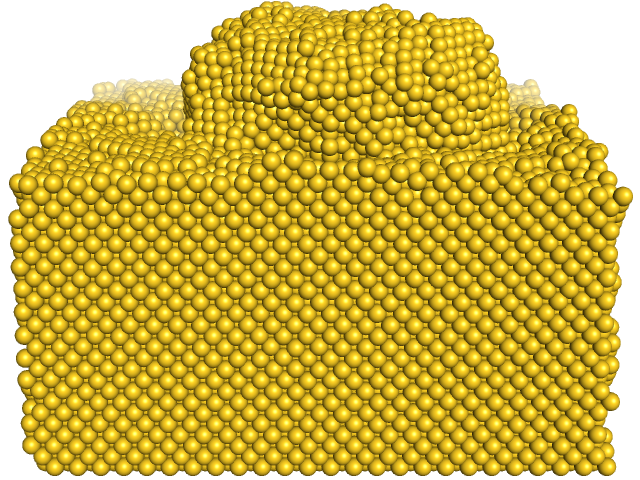
\includegraphics[width=\textwidth]{Au_deposition_tip60}
    \subcaption{Fortsetzung der Spitze ($\sigma_z = \SI{8.0}{\angstrom}$)}
    \label{fig:golddepositions-f}
  \end{subfigure}
  \caption[Gold-Abscheidung auf strukturierten Substraten]{
    Goldschicht nach 50 Abscheidungsschritten (\SI{47}{\angstrom}) auf verschiedenen Substraten
  }
  \label{fig:golddepositions}
\end{figure}

\begin{figure}[p]
  \captionsetup[subfigure]{singlelinecheck=false}
  \def\subfigwidth{0.49\textwidth}

  \begin{subfigure}[t]{\subfigwidth}
    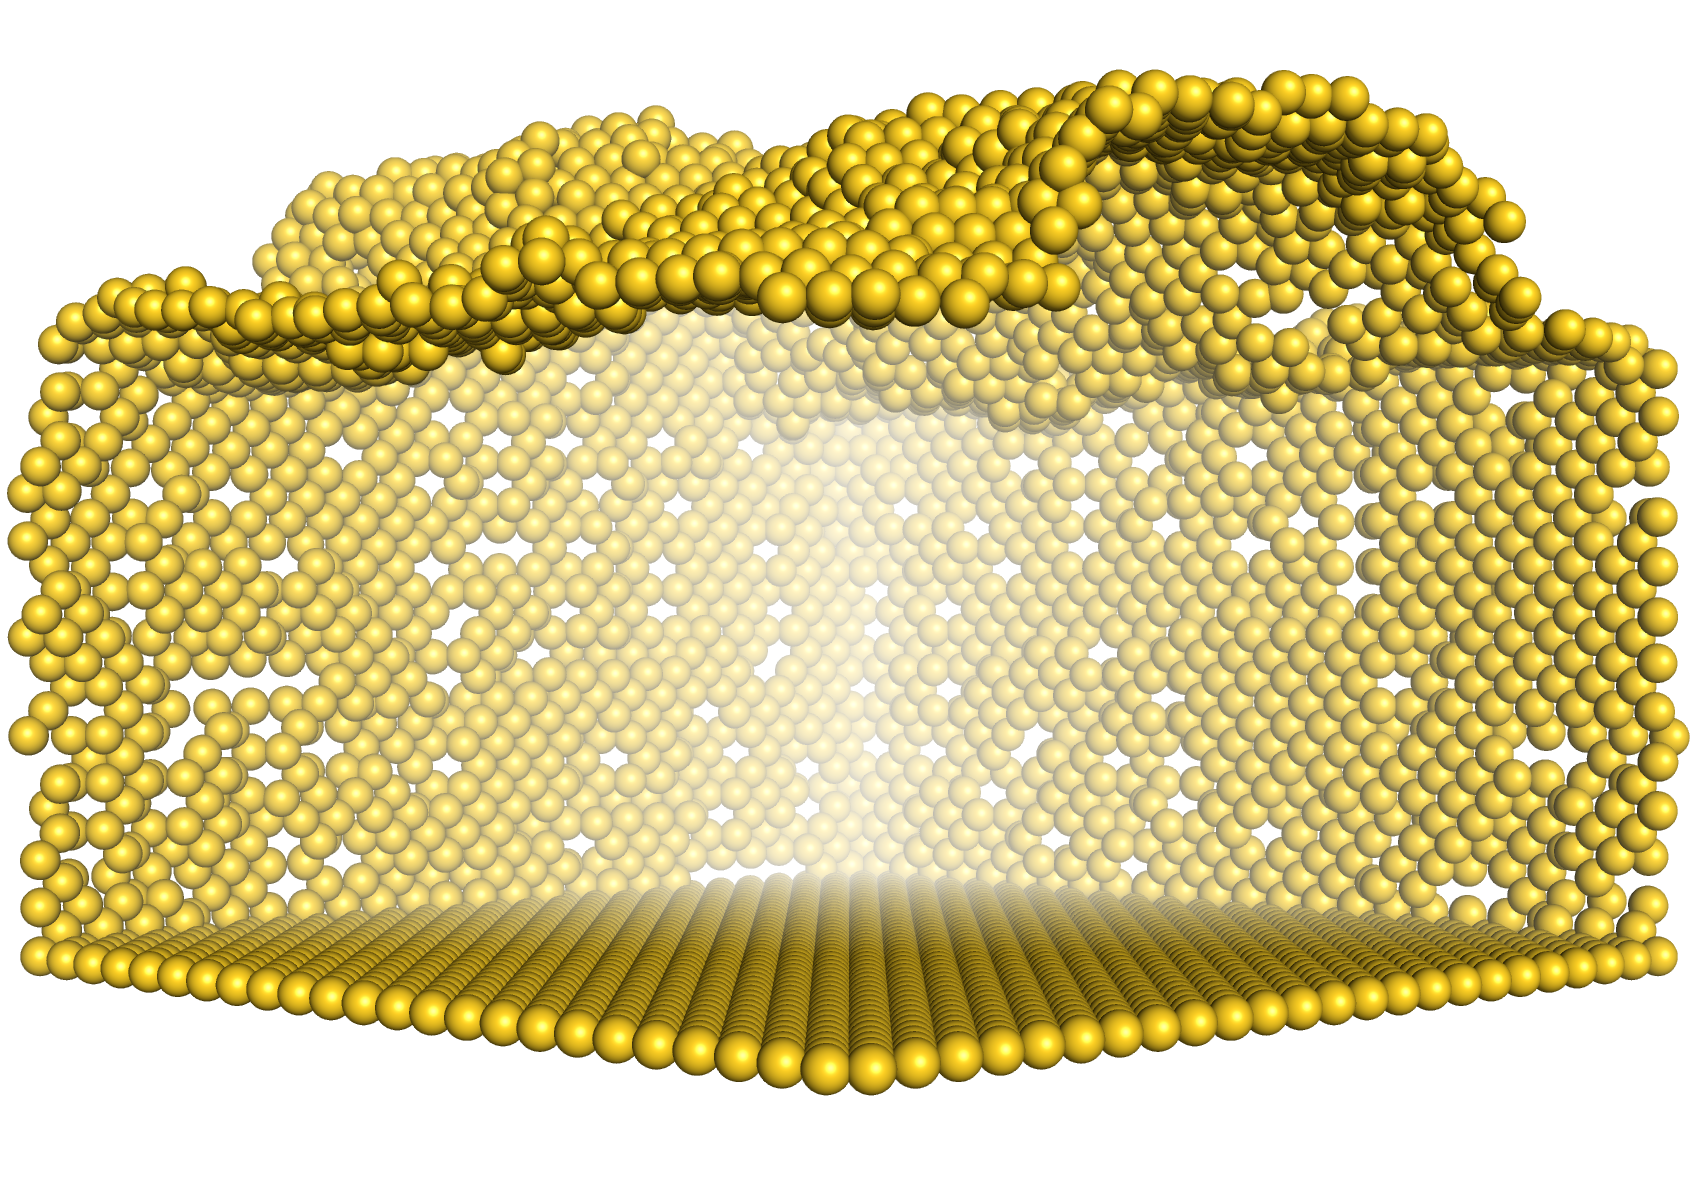
\includegraphics[width=\textwidth]{gold_step30_pockets}
    \subcaption{\SI{30}{\degree}-Stufe: Keine Poren oder Einschlüsse}
    \label{fig:goldpockets-a}
  \end{subfigure}
  \hfill
  \begin{subfigure}[t]{\subfigwidth}
    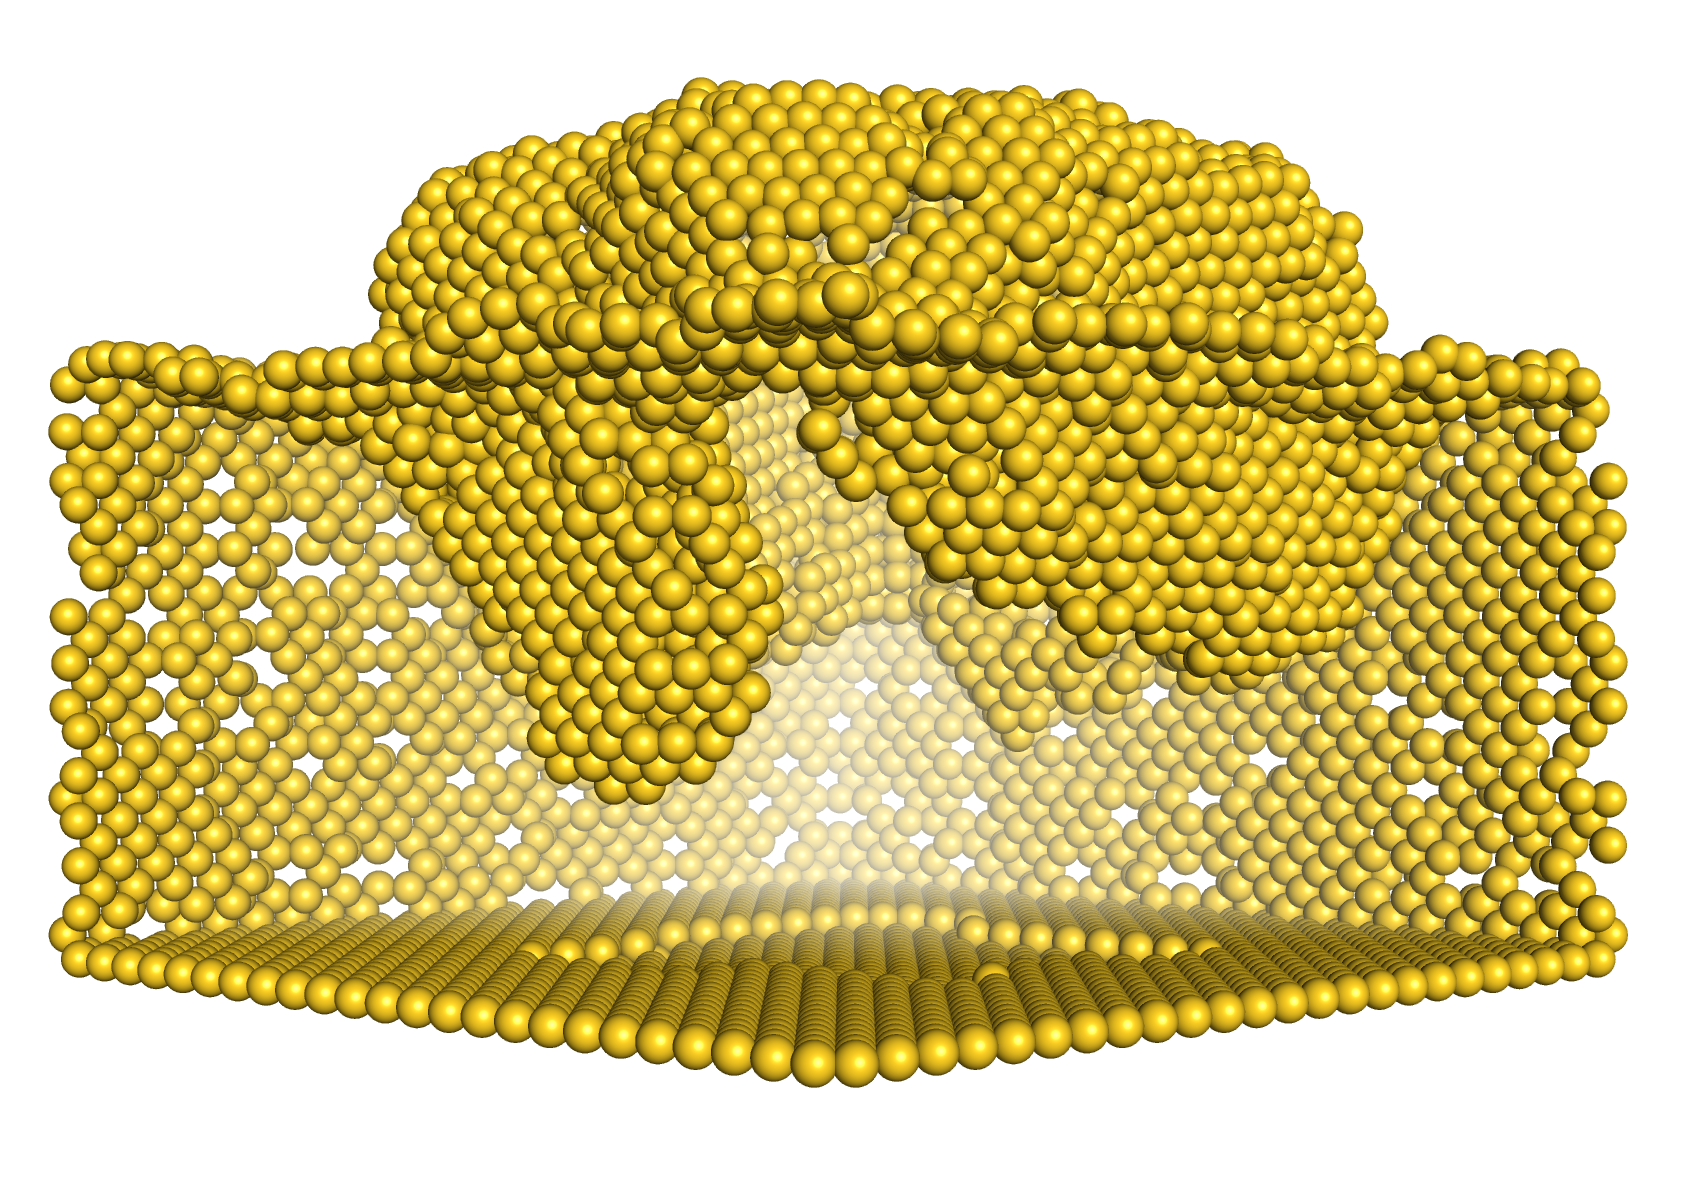
\includegraphics[width=\textwidth]{gold_tip90_pockets}
    \subcaption{Porenbildung an der Basis der \SI{90}{\degree}-Spitze}
    \label{fig:goldpockets-b}
  \end{subfigure}

  \caption[Porenbildung bei Gold-Strukturen]{Porenbildung bei Gold-Strukturen nach 40 Abscheidungsschritten (ca. \num{22000} PVD-Ereignisse $\hat{=}$ \SI{38}{\angstrom}).
  }
  \label{fig:goldpockets}
\end{figure}

Wie man den Alpha-Formen der simulierten Strukturen (Abbildung \ref{fig:goldpockets-a}) entnehmen kann, beinhaltet das abgeschiedene Gold bei geringen Neigungswinkeln keine Kristalldefekte, Poren oder Einschlüsse.
Bei Abscheidungen auf Substrate hoher Neigungswinkel (>\SI{60}{\degree}) bilden sich Poren mit größerer Ausdehnung (>\SI{20}{\angstrom}).
Durch Bildung von Überhängen an den Stufen werden die Poren zu Hohlräumen abgeschlossen, die nicht durch Relaxierung geschlossen werden.
Dies zeigt sich auch in den Oberflächenrauheiten der untersuchten Strukturen (Abbildung \ref{fig:goldroughness}).
Dabei wurden auch die Lamellen (Fins) und Gitter (Pillars) mit einer Strukturbreite von \SI{16}{\angstrom} untersucht, die innerhalb weniger Schritte aufgrund ihrer geringen Ausdehnung von \num{4} Atomdurchmessern durch Relaxierungseffekte verschwinden (Abbildung \ref{fig:goldroughness}).
Die Rauheit $\sigma_z$ wird über die per periodische Alpha-Form bestimmte Oberfläche des Systemes inklusive der Poren berechnet und somit bei großen Poren überschätzt.
\todo{welche effekte?}Die selben Effekte sollten auch bei größeren Strukturen zu beobachten sein.
Wie man jedoch Abbildung \ref{fig:goldroughness-b} entnehmen kann, lässt sich das nur andeutungsweise bei der \SI{45}{\degree}-Spitze beobachten.

Hier zeigt sich ein künstliches \todo{besserer Begriff}Artefakt der Simulationsmethode, die auf zusätzliche Relaxationen verzichtet und in z-Richtung abgeschirmte Teile der Oberfläche ignoriert.
Eine mögliche Lösung wäre die explizite Parametrisierung per Delaunay-Triangulation, wie sie in Abschnitt \ref{datadelaunay} diskutiert wurde.

\todo[inline]{Vergleich mit realistischer RMS von Gold-PVD (Faktor 10 höher: 3 Bindungslängen statt subatomar)}
\todo[inline]{Verringerung der Rauheit mit Sputterdauer}
\todo[inline]{Unterbinden von Nanopartikeln durch MD-Box}
\todo[inline]{kleine Nanopartikel wachsen bei Annealing, weil Schmelzpunkt geringer}
\todo[inline]{Finite-Size-Effekte führen zu Begrenzung des RMS-Wertes. Hier nicht untersucht.}
Svorcik et al.\cite{svorcik_annealing_2011}

\begin{figure}[bth]
  \captionsetup[subfigure]{singlelinecheck=false}
  \def\subfigwidth{0.49\textwidth}

  \begin{subfigure}[t]{\subfigwidth}
    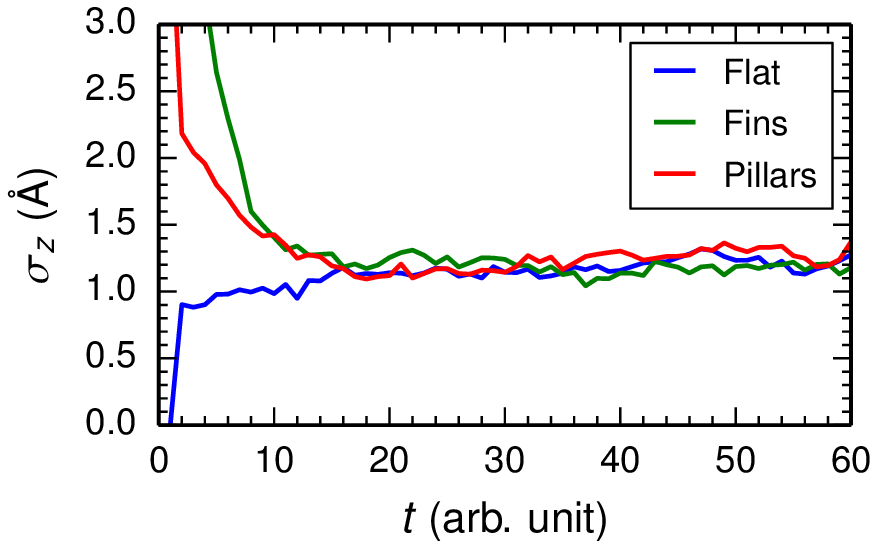
\includegraphics[width=\textwidth]{gold_goodroughness}
    \subcaption{Zeitverlauf der Rauheit von glatten (Flat) und fein strukturierten Oberflächen (Fins, Pillars: \SI{10}{\angstrom} breite Erhebungen)}
    \label{fig:goldroughness-a}
  \end{subfigure}
  \hfill
  \begin{subfigure}[t]{\subfigwidth}
    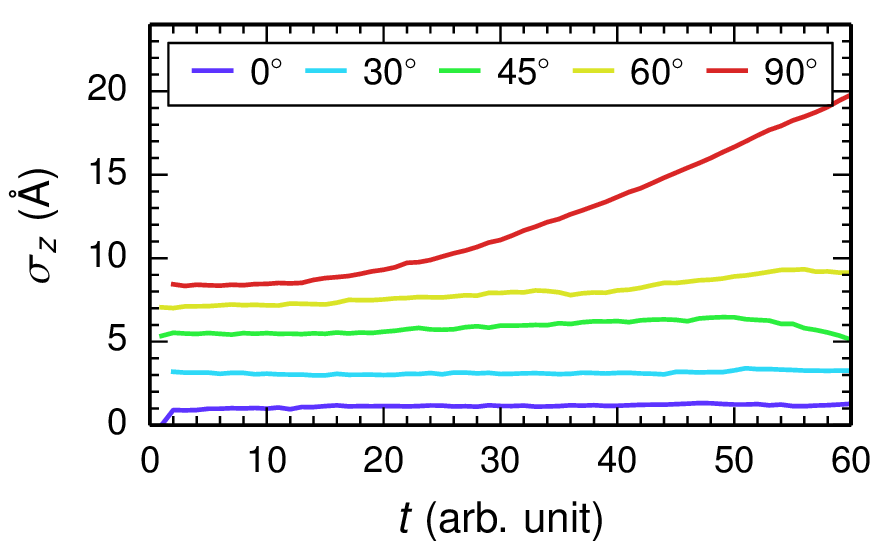
\includegraphics[width=\textwidth]{gold_tiproughness}
    \subcaption{Zeitverlauf der Rauheit von \SI{50}{\angstrom} breiten Spitzen variabler Steigung.
      Oberflächenrauheiten werden nicht verringert
    }
    \label{fig:goldroughness-b}
  \end{subfigure}

  \caption[Oberflächenrauheit von Gold]{Oberflächenrauheit von Gold.
    Im idealen Fall konvergiert die Rauheit gegen einen konstanten Wert von \SI{1.2}{\angstrom}
  }
  \label{fig:goldroughness}

\end{figure}

\subsection{Skalierbarkeit der Rechenzeit mit der Simulationsgröße}

Zur Untersuchung der Skalierbarkeit wurden Substratbreiten von \SI{100}{\angstrom}, \SI{200}{\angstrom}, \SI{1000}{\angstrom} und \SI{10000}{\angstrom} und \SI{20000}{\angstrom} auf Atomzahl und Laufzeit untersucht (Tabelle \ref{tab:goldscalability}).


\begin{table}[hbp]

  \caption[asd]{Untersuchungen zur Skalierbarkeit des Systemes}
  \label{tab:goldscalability}

  \begin{tabularx}{\textwidth}{|Xrrrrr|}
    \hline
    \textbf{Größe} & \textbf{Atome} & \textbf{Ereignisse} & \textbf{Schritte} & \textbf{Worker} & \textbf{Laufzeit} \\
    \hline
    \SI{106x106}{\angstrom}      &  \num{59549}      &  \num{46030}     &  \num{100}  &  \num{4}   &  \SI{116042}{\second}  (\SI{1.3}{\day})  \\
    \SI{204x204}{\angstrom}      &  \num{152374}     &  \num{102374}    &  \num{100}  &  \num{18}  &  \SI{91680}{\second}   (\SI{1.1}{\day})  \\
    \SI{500x500}{\angstrom}      &  \num{1708600}    &  \num{1401081}   &  \num{100}  &  \num{50}  &  \SI{264900}{\second}  (\SI{3.1}{\day})  \\
    \SI{1000x1000}{\angstrom}    &  \num{1591908}    &  \num{381588}    &  \num{24}  &  \num{46}  &  \SI{5340}{\second}    (\SI{0.1}{\day})  \\
    \SI{10000x10000}{\angstrom}  &  \num{128433070}  &  \num{8186990}   &  \num{8}    &  \num{46}  &  \SI{422820}{\second}  (\SI{4.9}{\day})  \\
    \SI{20000x20000}{\angstrom}  &  \num{490948111}  &  \num{10356031}  &  \num{2}    &  \num{46}  &  \SI{422820}{\second}  (\SI{4.9}{\day})  \\
    \SI{20000x20000}{\angstrom}  &  \todo[inline]{neuewerte}\num{-1}  &  \num{10356031}  &  \num{2}    &  \num{46}  &  \SI{422820}{\second}  (\SI{4.9}{\day})  \\
    \hline
  \end{tabularx}
\end{table}
